\section{Excitation et détection d'atomes de Rydberg près d'une puce}

\noindent Cette diversité de nuages atomiques nous permet d'exciter des atomes de Rydberg dans différentes conditions de densité atomique, de température et de distance à la puce.
Nous présentons dans le reste de ce chapitre la partie de notre dispositif expérimental servant à exciter, détecter et manipuler les atomes de Rydberg.
Notre dispositif est particulier dans la mesure où tout ce que concerne les niveaux de Rydberg a lieu près d'une surface conductrice, ce qui rend les choses plus difficiles.

Après avoir donné le principe de l'excitation à deux photons des niveaux de Rydberg et de la détection par ionisation sélective, nous ferons une présentation de rapide de l'effet Strak et de ses effets sur nos expériences.
Nous décrirons ensuite les techniques mises en place afin de contrôler les champs électriques près de la puce.
Nous finirons ce chapitre par une présentation de la technique de spectroscopie microonde des niveaux de Rydberg et de son utilisation pour mesurer les champs électriques résiduels.

	\subsection{L'excitation à deux photons des atomes de Rydberg}

\noindent Les atomes de rubidium piégés dans un nuage près de la puce sont excités vers les niveaux de Rydberg par une transition laser à deux photons désaccordée par rapport au niveau intermédiaire.
Dans nos recherches, deux niveaux de Rydberg différents ont été excités par laser à partir de l'état fondamental 5S$_{1/2}$ : le niveau 60S$_{1/2}$ et le niveau 50D$_{3/2}$.
Nous décrivons ici l'excitation d'un nuage d'atomes de Rydberg au sein d'un nuage froid dans le piège magnétique, en négligeant les interactions entre atomes de Rydberg et en nous concentrant sur le niveau $\mathrm{60S_{1/2}}$.

La transition du niveau fondamental au niveau de Rydberg est faite par l'absorption d'un photon rouge à $\lambda = \SI{780}{\nano\meter}$, désaccordé de $\delta=+\SI{540}{\MHz}$ par rapport à la transition $\mathrm{5S_{1/2},F=2 \rightarrow 5P_{3/2},F'=3}$, et d'un photon bleu à $\lambda = \SI{480}{\nano\meter}$, accordé pour satisfaire la condition de résonance vers le niveau choisi.
La figure \eqref{fig:2photons} représente le schéma de niveaux de l'excitation du niveau $\mathrm{60S_{1/2}}$.
Les deux faisceaux d'excitation sont superposés et se propagent selon la direction $+x$. Leurs polarisations sont définies par rapport à l'axe de quantification des niveaux atomiques, déterminé par le champ magnétique de biais $B_x$ dans le fond du piège.
La figure \eqref{fig:lasers_excit} représente la géométrie des faisceaux laser d'excitation.
Dans cette configuration, seul le sous-niveau $m_j=+1/2$ du niveau 60S est excité.
%
\begin{figure}[!h]
\centering
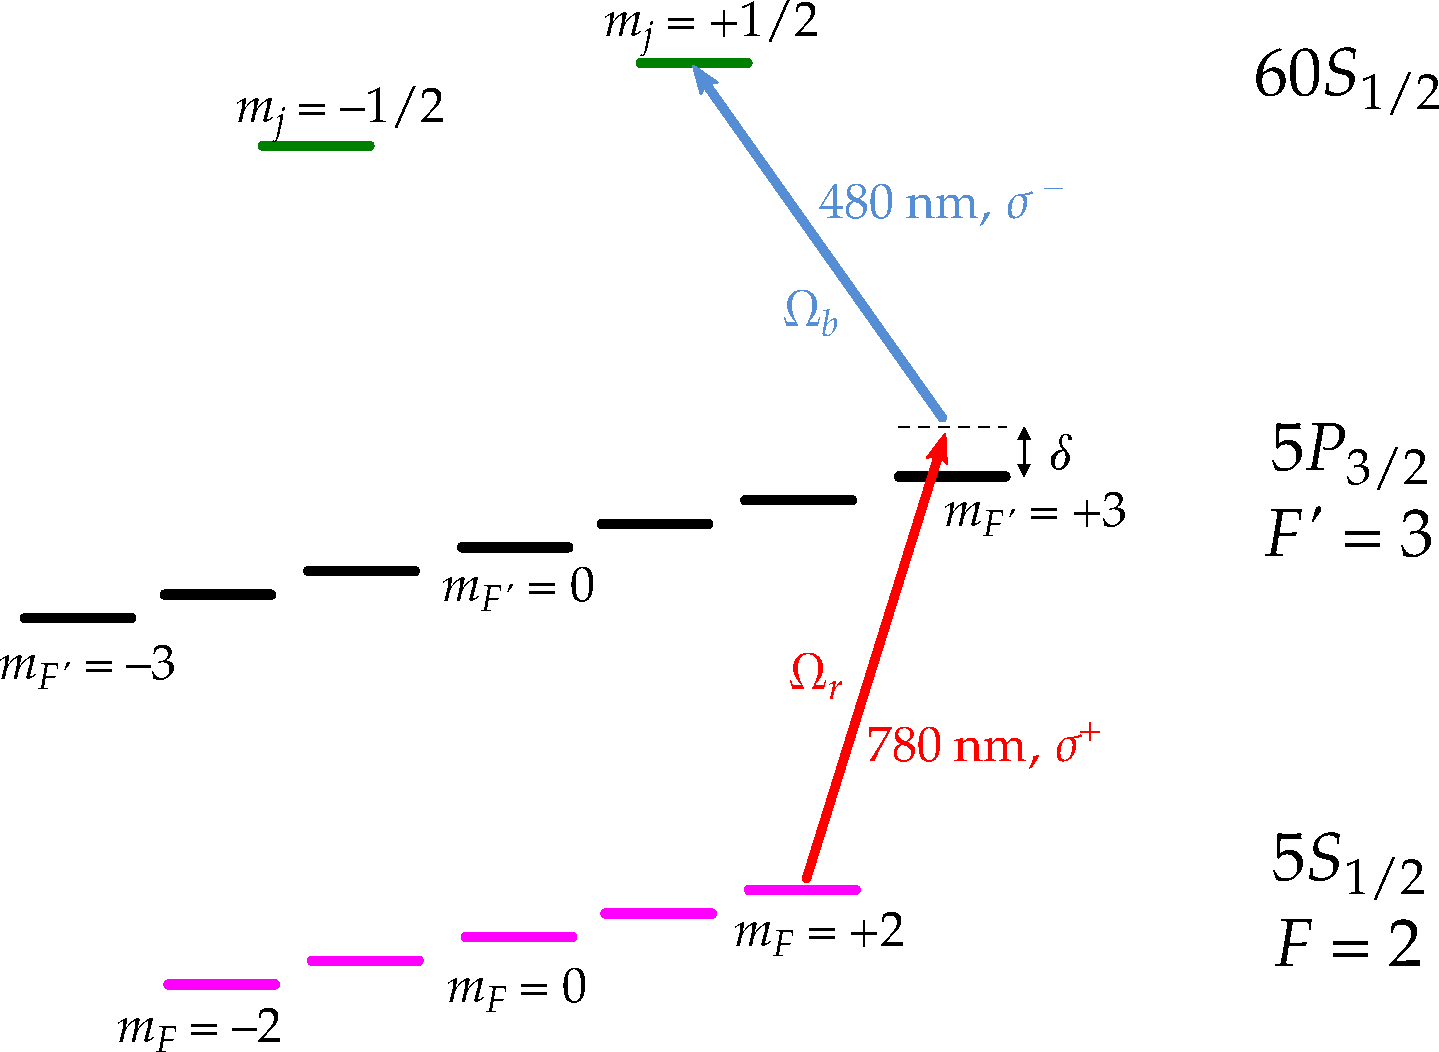
\includegraphics[width=.8\linewidth]{figures/2photons}
\caption[Excitation du niveau 60S]{Schéma de l'excitation laser du niveau 60S, à partir d'atomes de \Rb{87} dans le niveau fondamental dans le piège magnétique.
La polarisation de chaque laser est indiquée.
$\Omega_r$ et $\Omega_b$ sont les fréquences de Rabi des transitions à \num{780} et \SI{480}{\nano\meter} respectivement.
$\delta=\SI{540}{\MHz}$ est le désaccord par rapport au niveau intermédiaire.
}
\label{fig:2photons}
\end{figure}

Le faisceau rouge a typiquement un col de $\SI{150}{\um}$ et une puissance de $\SI{50}{\micro\watt}$ au niveau des atomes.
Le laser rouge est désaccordé de $\delta=\SI{540}{\MHz}$ par rapport à la transition $ \ket{\mathrm{5S_{1/2},F=2,m_F=+2}} \rightarrow \ket{\mathrm{5P_{3/2},F'=3,m_F'=+3}}$, dont le moment de transition dipolaire vaut $\SI{2.98931 (62)} ea_0$ \cite{DATA_STECKRB87}.
D'après les caractéristiques du faisceau, la fréquence de Rabi correspondant à cette transition est de l'ordre de $\Omega_r \simeq 2\pi\times \SI{40}{\MHz}$.
Le taux d'émission spontanée de photons rouge par le niveau intermédiaire, de durée de vie $\Gamma^{-1} \simeq \SI{26}{\ns}$, est donné par
\begin{equation}
\label{eq:scattering_5P3/2}
\Gamma_{sp} = \frac{1}{2} \frac{\Omega_r^2 \Gamma}{\delta^2 + \Omega_r^2 + \Gamma^2}
\simeq \frac{\Omega_r^2}{2\delta^2} \Gamma,
\end{equation}
où $\Gamma = 2\pi \times 6.065 MHz$ est la largeur naturelle du niveau $\mathrm{5P_{3/2}}$.
La dernière égalité est vérifiée dans l'approximation $\delta^2 \gg \Omega_r^2, \Gamma^2$, qui est ici valide.
Avec nos valeurs d'intensité et de désaccord du laser, on obtient $\Gamma_{sp} \simeq \num{2.5e-3} \Gamma = 2\pi\times \SI{0.657}{\MHz}$, ce qui correspond à l'émission d'un photon  toutes les $\Gamma_{sp}^{-1} = \SI{0.24}{\us}$.
Or lorsqu'un atome absorbe et ré-émet un tel photon, il gagne une énergie moyenne
$\Delta E = p^2/(2m_{Rb87}) = h^2/(2m_{Rb87} \lambda^2) = \SI{180}{\nano\kelvin} / \kb$.
Le piège est ainsi chauffé par le laser rouge d'excitation, ce qui limite à la fois la puissance que l'on peut envoyer sur le nuage, et le nombre d'impulsions laser d'exciation que l'on peut faire subir à un même nuage sans l'altérer.

Le faisceau bleu a typiquement un col de $\SI{22}{\um}$ et une puissance estimée à $\SI{4}{\milli\watt}$ au niveau des atomes.
Le moment dipolaire de la transition $ \ket{\mathrm{5P_{3/2},F'=3,m_F'=+3}} \rightarrow \ket{\mathrm{60S_{1/2},m_j=+1/2}}$ est cependant bien plus faible que le précédent, et vaut $\SI{9.9e-3} ea_0$
\footnote{Nous rappelons ici que, comme nous l'avons mentionné en \ref{sec:alkalRydberg}, le bon nombre quantique magnétique pour les niveaux de Rydberg est $m_j$ et non pas $m_F$.}.
La fréquence de Rabi pour cette transition est alors de $\Omega_b = 2\pi\times \SI{8}{\MHz}$.
Les fréquences de Rabi des deux trasitions satisfont l'approximation $\Omega_{r,b} \ll \delta$, ce qui nous permet de négliger l'occupation du niveau intermédiaire, et donc de l'éliminer adiabatiquement \cite{TXT_ASPECTFABRE_QUANTOPT}.
Le système à trois niveaux se ramène alors à un système effectif à deux niveaux, couplés par une fréquence de Rabi
\begin{equation}
\label{eq:Rabi_2photons}
\Omega = \frac{\Omega_r \Omega_b}{\delta}.
\end{equation}
Avec nos paramètres, on obtient une fréquence de Rabi $\Omega = 2\pi \times \SI{296}{\kHz}$ pour la transition $\ket{\mathrm{5S_{1/2},F=2,m_F=+2}} \rightarrow \ket{\mathrm{60S_{1/2},m_j=+1/2}}$.
Ce paramètre peut être varié simplement en ajustant la puissance du laser rouge ou la puissance du laser bleu.

%
\begin{figure}[!h]
\centering
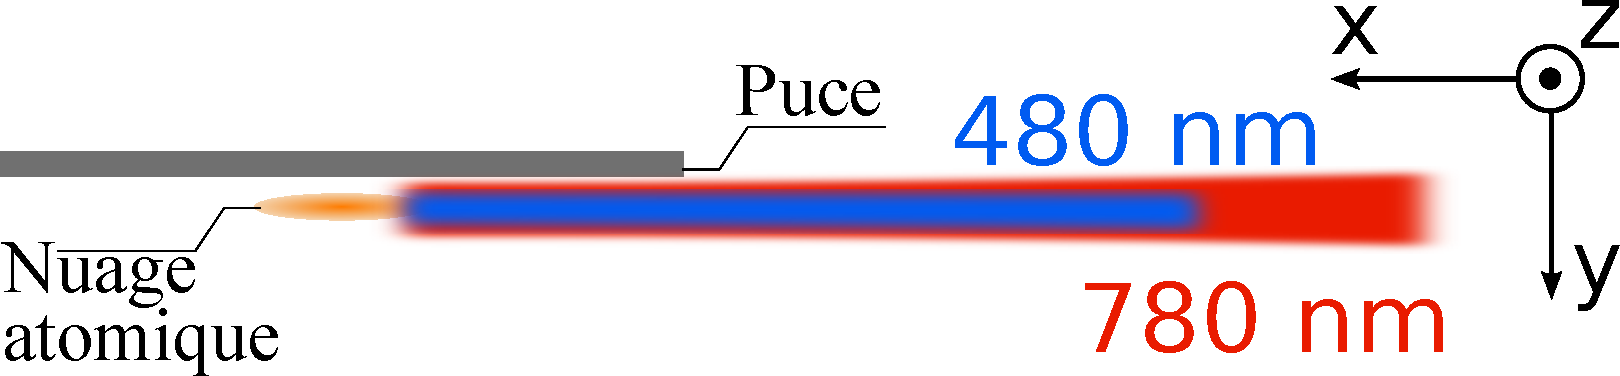
\includegraphics[width=.8\linewidth]{figures/lasers_excit}
\caption[Faisceaux laser pour l'excitation des Rydberg]{Schéma représentant la géométrie des faisceaux laser d'excitation.
}
\label{fig:lasers_excit}
\end{figure}

		
	\subsection{La détection par ionisation des atomes de Rydberg}\label{subsec:detection}
\noindent L'électron de valence d'un atome de Rydberg alcalin est très proche du seuil d'ionisation.
Il est donc très facile de l'arracher au noyau en appliquant un champ électrique.
Nous exploitons cette caractéristique pour détecter les atomes de Rydberg par ionisation en champ électrique :
une fois l'atome ionisé, le c\oe ur atomique est accéléré par des électrodes vers un détecteur à avalanche (Channeltron).


%
\begin{figure}[h]
\centering
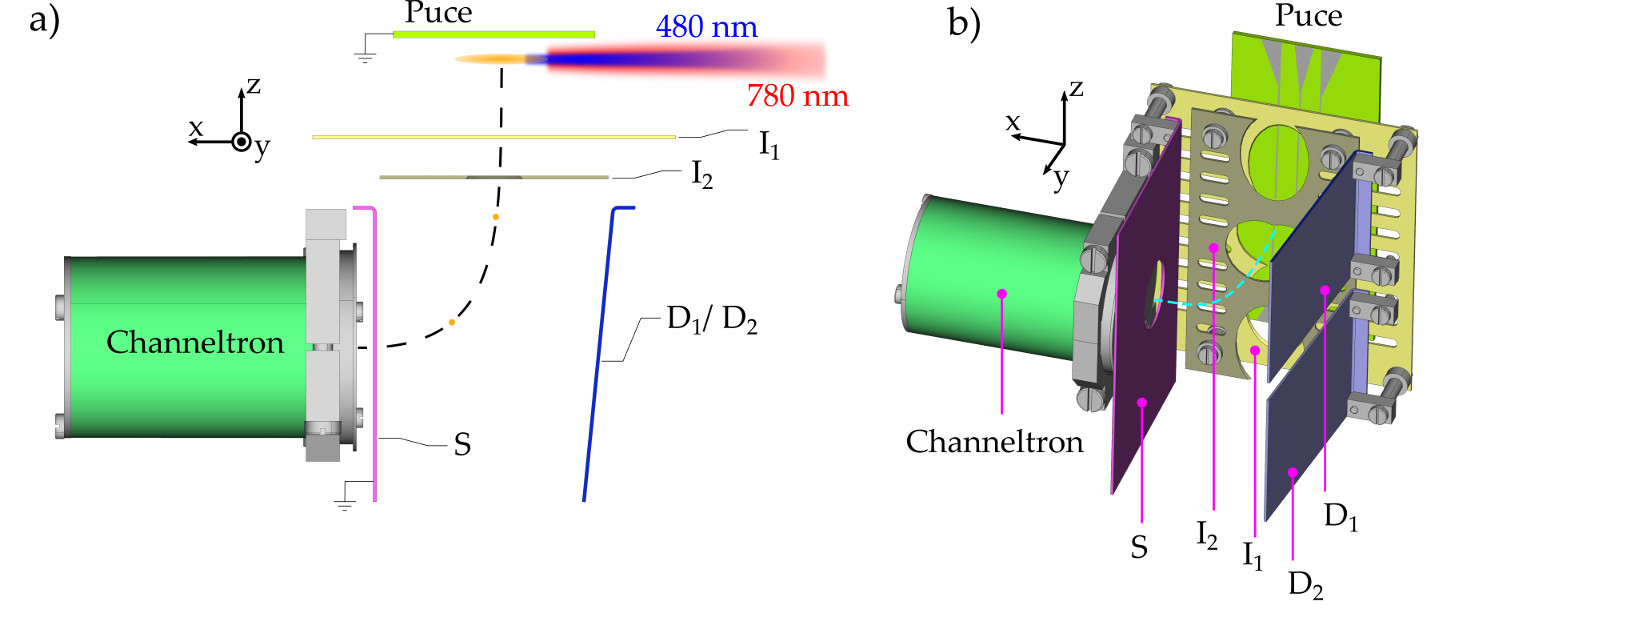
\includegraphics[width=\linewidth]{figures/schema_detect}
\caption[Système de détection des atomes de Rydberg]{Schéma représentant le système de détection des atomes de Rydberg.
\textbf{a)} vu de dessus et \textbf{b)} en projection axonométrique.
Après excitation, les atomes de Rydberg sont ionisés par les élctrodes $I_1$ et $I_2$.
Les ions ainsi créés et accélérés sont défléchis par les électrodes $D_1$ et $D_2$, en direction du détecteur Channeltron.
L'électrode $S$ est mise à la masse et sert à écranter la tension présente à l'entrée du Channeltron.
La trajectoire des ions est indiquée en lignes pointillées et les faisceaux lasers d'excitation sont représentés en \textbf{a)}.
}
\label{fig:schema_detect}
\end{figure}
%
La figure \eqref{fig:schema_detect} présente un schéma détaillé du système de détection par ionisation.
Au moment de la détection, une tension négative est appliquée sur les électrodes d'ionisation $I_1$ et $I_2$.
La tension sur ces électrodes crée un champ électrique au niveau des atomes, la puce étant mise à la masse.
Ce champ électrique ionise les atomes de Rydberg et accélère les ions positifs ainsi créés.
Ces ions sont ensuite défléchis en direction du Channeltron par les électrodes $D_1$ et $D_2$, chargées en permanence à une tension $V_{defl} = +\SI{150}{\V}$.
Une grille placée à l'entrée du Channeltron est alimentée par une tension de $\SI{-3000}{\V}$.
Une électrode trouée mise à la masse est placée devant cette grille afin d'écranter les $\SI{-3000}{\V}$ pour la région de piégeage des atomes.
Lorsque les ions arrivent dans le Channeltron, celui-ci génère par avalanche un signal électronique qui est envoyer vers un amplificateur et un discriminateur permettant de décompter les ions détectés.
Le Channeltron est isolé thermiquement et chauffé à une température de $\SI{42}{\K}$ afin d'augmenter son efficacité.

\subsubsection*{Sélectivité de niveau de la détection par ionisation}
\noindent Chaque atome de Rydberg présente une énergie différente, telle que discutée en \ref{sec:alkalRydberg}.
Cela signifie qu'ils sont tous à une distance différente du seuil d'ionisation, et \textit{in fine} que chaque niveau de Rydberg sera ionisé pour une valeur de champ électrique spécifique.
L'on peut ainsi appliquer une rampe de tension sur les électrodes d'ionisation, afin que chaque niveau de Rydberg soit ionisé à un instant différent.
Alors, les ions correspondants arriveront à des instants différents au Channeltron et pourront être distingués.
La figure \eqref{fig:arrTimes6057} montre un signal de détection sélective des niveaux de Rydberg $\mathrm{60S_{1/2}}$ et $\mathrm{57S_{1/2}}$.
La rampe de tension et les fenêtres temporelles de détection sont optimisées afin de distinguer au mieux les différents niveaux de Rydberg détectés.
L'efficacité de détection de notre dispositif a été mesurée à $\SI{90}{} \pm \SI{10}{\percent}$.
%
\begin{figure}[h]
\centering
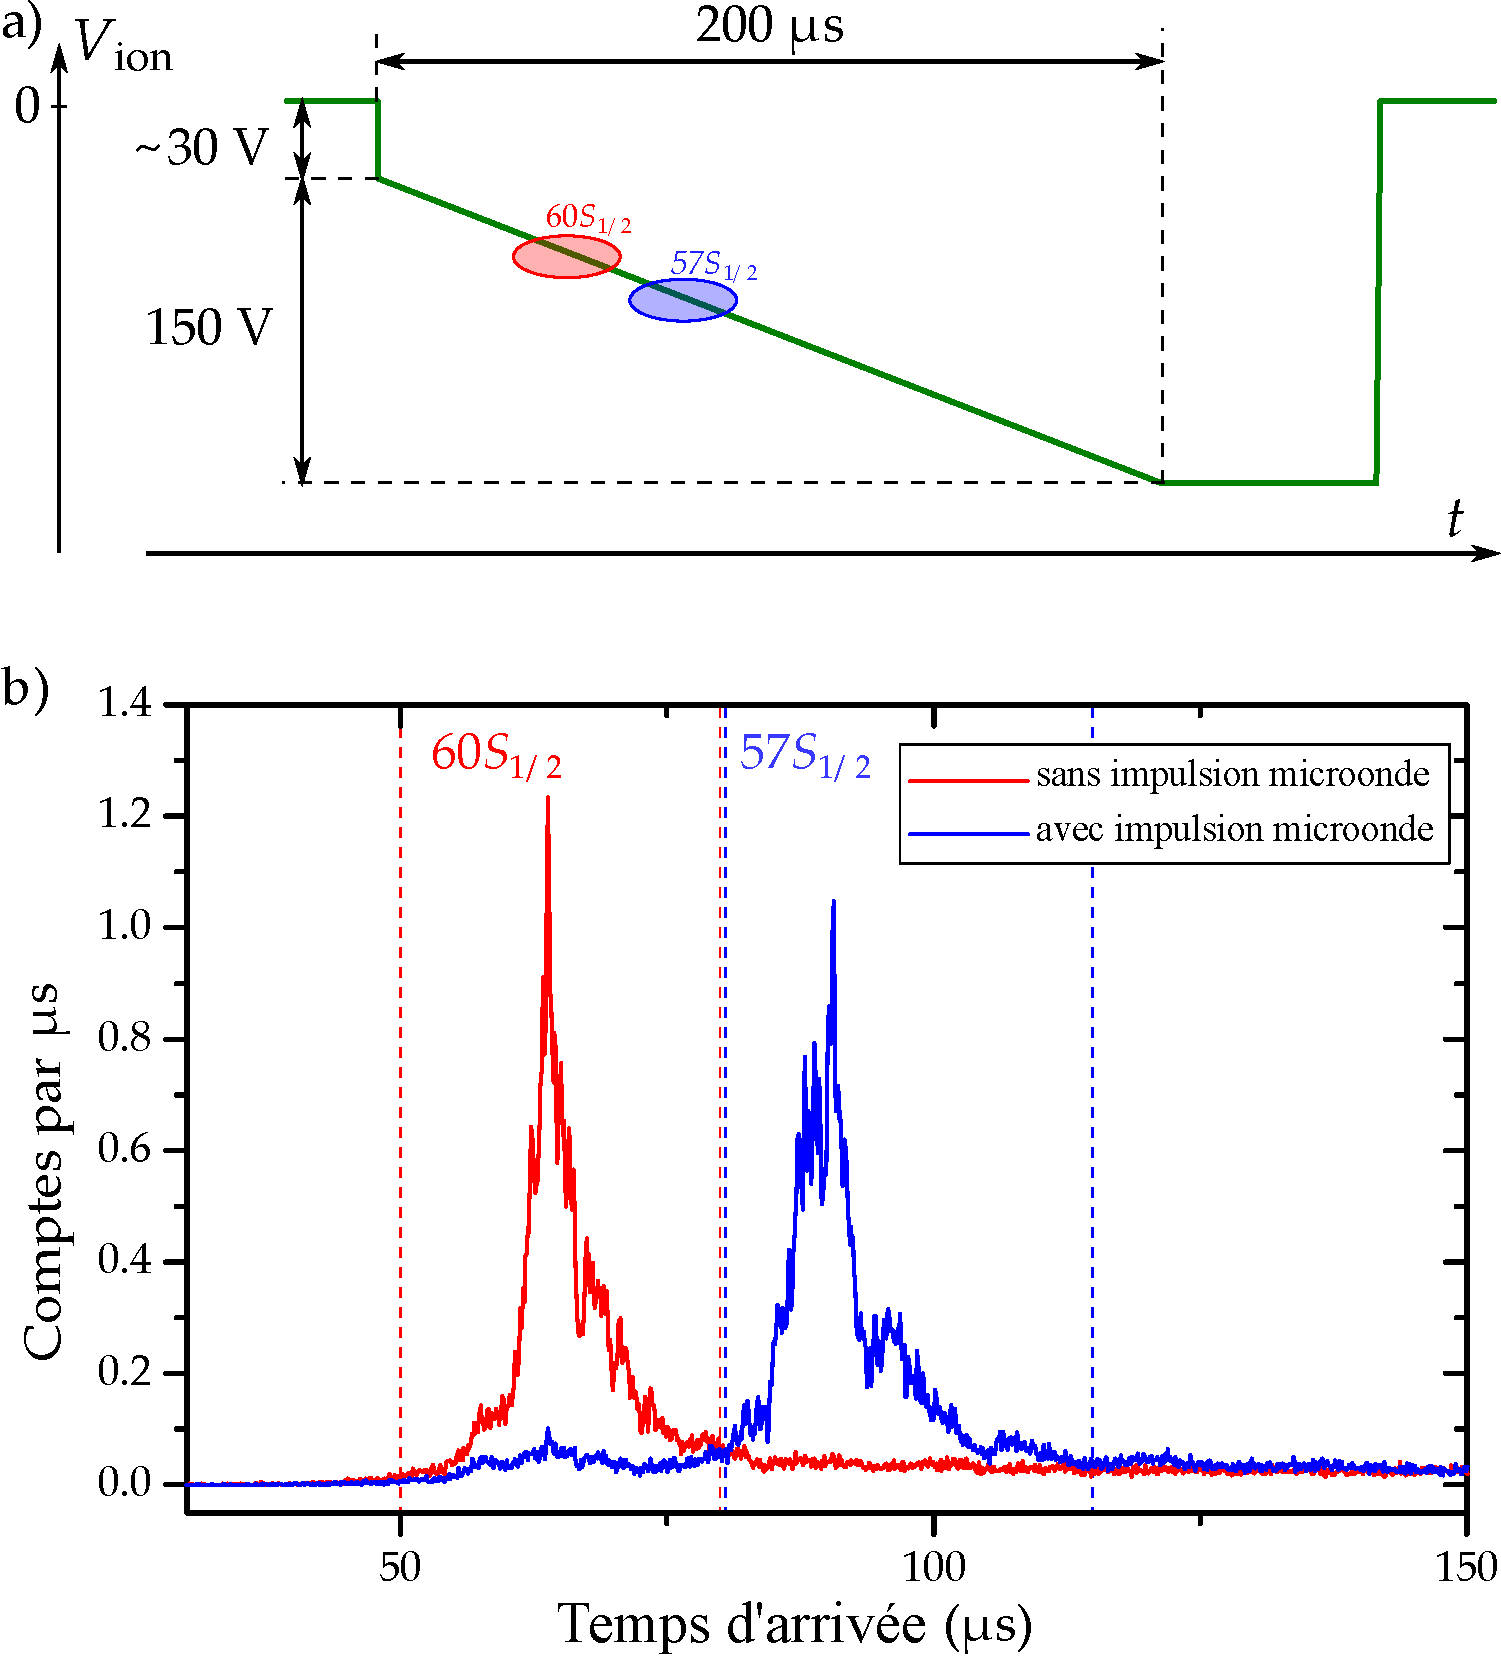
\includegraphics[width=.7\linewidth]{figures/arrTimes6057}
\caption[Détection sélective des niveaux $\mathrm{60S_{1/2}}$ et $\mathrm{57S_{1/2}}$]{
Détection sélective des atomes de Rydberg.
\textbf{a)} une rampe de tension $V_{ion}$ typique appliquée sur les électrodes d'ionisation.
Les seuils d'ionisation des niveaux $\mathrm{60S_{1/2}}$ et $\mathrm{57S_{1/2}}$ sont indiqués en rouge et bleu respectivement.
\textbf{b)} Temps d'arrivée des ions correspondants. Des fenêtres temporelles de détection, représentées en pointillés, sont définies pour compter sélectivement les atomes dans les niveaux $\mathrm{60S_{1/2}}$ et $\mathrm{57S_{1/2}}$.
Les atomes sont préparés dans l'état $\mathrm{60S_{1/2}}$ et le niveau $\mathrm{57S_{1/2}}$ est peuplé par une impulsion $\pi$ de la transition microonde adéquate.
Les échelles de temps sont différentes en \textbf{a)} et \textbf{b)}.
}
\label{fig:arrTimes6057}
\end{figure}
%


%EJECTE : note sur l'ionisation diabatique vs adiabatique. 
		
	\subsection{Les champs électriques parasites, défi des atomes de Rydberg sur puce}\label{subsec:flashRb}
	%problème des champs électriques et flash de Rb}
\noindent Comme nous l'avons dit au chapitre \ref{chapter:Rydberg}, les atomes de Rydberg sont des objets extrêmement sensibles au champ électromagnétique.
Or, dans notre expérience, nous souhaitons exciter et manipuler des atomes de Rydberg à proximité immédiate d'une surface, la puce à atomes.
Les bruits électriques étant inévitables près d'une surface, la présence de la puce va rendre difficile l'excitation et la manipulation des atomes de Rydberg.

\subsubsection*{Premiers spectres}
\noindent Ce problème est très clair sur les premiers spectres que nous avons fait de la transition $\ket{\mathrm{5S_{1/2}}} \rightarrow \ket{\mathrm{60S_{1/2}}}$, présentés en figure \eqref{fig:vieilles_raies}.
%
\begin{figure}[h]
\centering
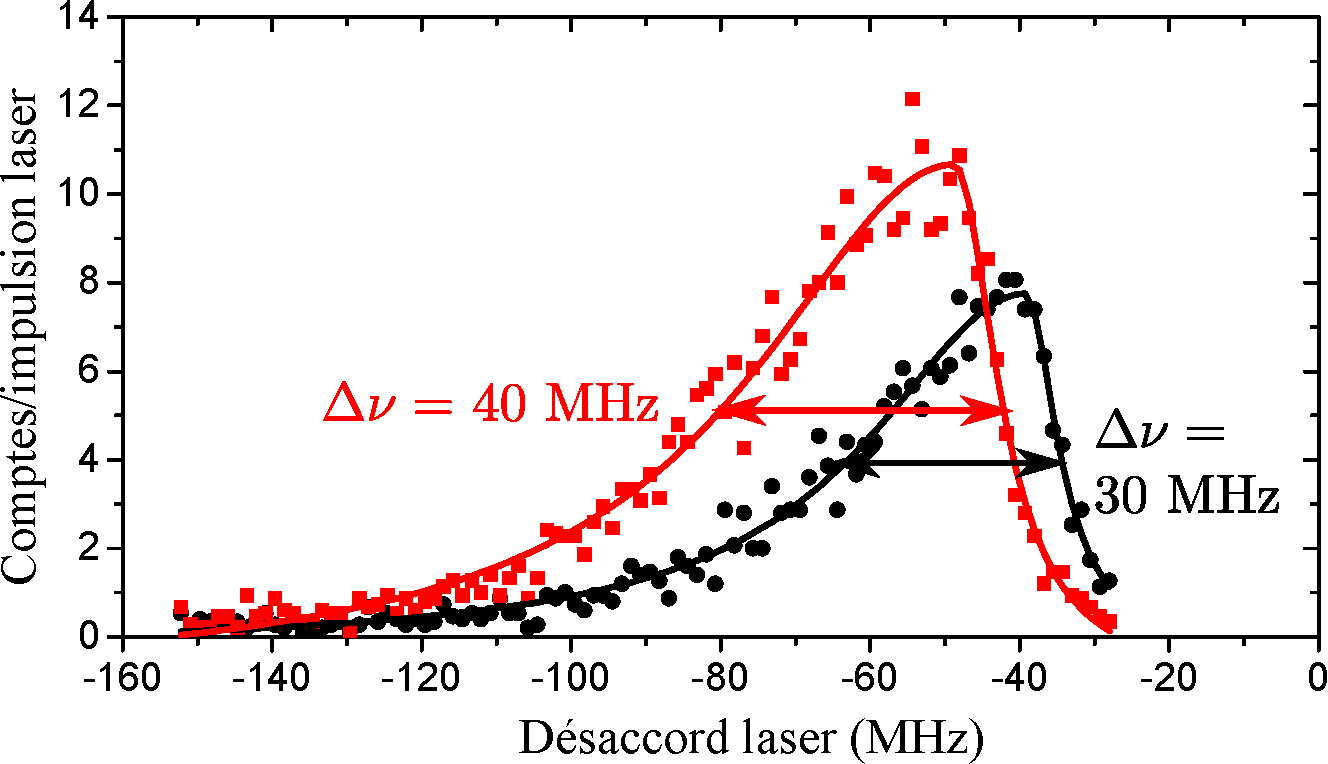
\includegraphics[width=.8\linewidth]{figures/vieilles_raies}
\caption[Spectres d'excitation laser 5S-60S avant le dépôt de rubidium sur la puce]{
Deux spectres laser de la transition $5\mathrm{S}\rightarrow60\mathrm{S}$, avant correction des inhomogénéités et de la dérive du champ électrique.
Leurs largeurs sont de $\SI{30}{\MHz}$ et $\SI{40}{\MHz}$ respectivement, et ils sont décalés en fréquence de $\SI{12}{\MHz}$ l'un par rapport à l'autre.
Les deux spectres ont été pris dans les mêmes conditions, à \SI{1}{\hour} d'intervalle, pendant laquelle un MOT était piégé devant la puce.
L'origine de l'axe des abscisses correspond à la fréquence résonante de la transition $\mathrm{5S}\rightarrow\mathrm{60S}$ en l'absence de champ électrique.
}
\label{fig:vieilles_raies}
\end{figure}
%
Ces premiers spectres présentent des largeurs de raie de plusieurs dizaines de $\si{\MHz}$, et une forme asymétrique caractéristique d'un élargissement Stark inhomogène.
De plus, une heure de fonctionnement de l'expérience cause un déplacement en fréquence de la raie de \SI{12}{\MHz}.

Cet effet est causé par la variation spatiale et temporelle du champ électrique dans la région du nuage atomique.
L'énergie des niveaux de Rydberg dépend fortement du champ électrique extérieur au niveau de chaque atome.
Ainsi, si les atomes dans différentes régions du nuage voient des champs électriques différents, la fréquence de la transition $\mathrm{5S}\rightarrow\mathrm{60S}$ sera déplacée différemment dans chaque région, et la raie spectrale s'en trouvera élargie.

	\subsubsection*{L'effet Stark}
\noindent Afin de comprendre ce phénomène plus en détail, attardons-nous à décrire l'effet Stark.
La présence d'un champ électrique constant $\vec{F}$ dans l'environnement ajoute au hamiltonien atomique un terme de couplage entre le champ et l'opérateur dipolaire électrique.
En présence d'un champ électrique, le hamiltonien devient
\begin{equation}
\label{eq:hamilt_Stark}
\hat{H} = \hat{H}_0 - \vec{\hat{d} \cdot F} = \hat{H}_0 + q~\vec{\hat{r}\cdot F},
\end{equation}
où $\hat{H}_0$ est le hamiltonien libre de l'atome, dont les énergies propres sont calculées par la théorie du défaut quantique selon l'équation \eqref{eq:E_I_delta}, $\hat{\vec{r}}$ l'opérateur position de l'électron dans le potentiel atomique et $q$ la charge élémentaire, supposée positive.

Le hamiltonien Stark \eqref{eq:hamilt_Stark} perd la symétrie sphérique de $\hat{H}_0$, au profit d'une symétrie cylindrique autour de l'axe défini par le vecteur de champ électrique $\vec{F}$.
Cet axe, que nous choisirons comme étant l'axe $(Oz)$, devient alors l'axe de quantification naturel du problème.
Dans la base construite autour de cet axe, le terme d'énergie Stark prend la forme
\begin{equation}
\label{eq:dipole_Stark}
\hat{H}_S = q\hat{z}|\vec{F}| = q\hat{r} \sqrt{\frac{4\pi}{3}} Y_1^0  |\vec{F}|.
\end{equation}
où $\hat{z}$ est la composante selon $z$ de l'opérateur position, $\hat{r}$ sa norme, et $Y_0^1$ l'harmonique sphérique $(l=0,m_l=1)$.
Ce hamiltonien ne couple que les états de même $m_l$ et vérifiant $\Delta l = \pm 1$.

Le calcul de l'effet Stark par diagonalisation du hamiltonien pour un niveau de Rydberg donné est alors simple à mener numériquement, en réduisant le sous-espace à considérer grâce à la règle de sélection $\Delta m_l = 0$.
Cette même règle de sélection permet d'imposer la condition $\Delta m_j= \Delta m_l + \Delta m_s = 0$, car l'effet Stark n'introduit aucun terme permettant de coupler des états de spins électroniques différents.
La figure \eqref{fig:Stark_60S} montre les énergies propres trouvées par diagonalisation du hamiltonien \eqref{eq:hamilt_Stark}, pour les états d'énergie proche de celle du niveau $\mathrm{60S_{1/2},m_j=1/2}$ et de même $m_j$.
%
\begin{figure}[!h]
\centering
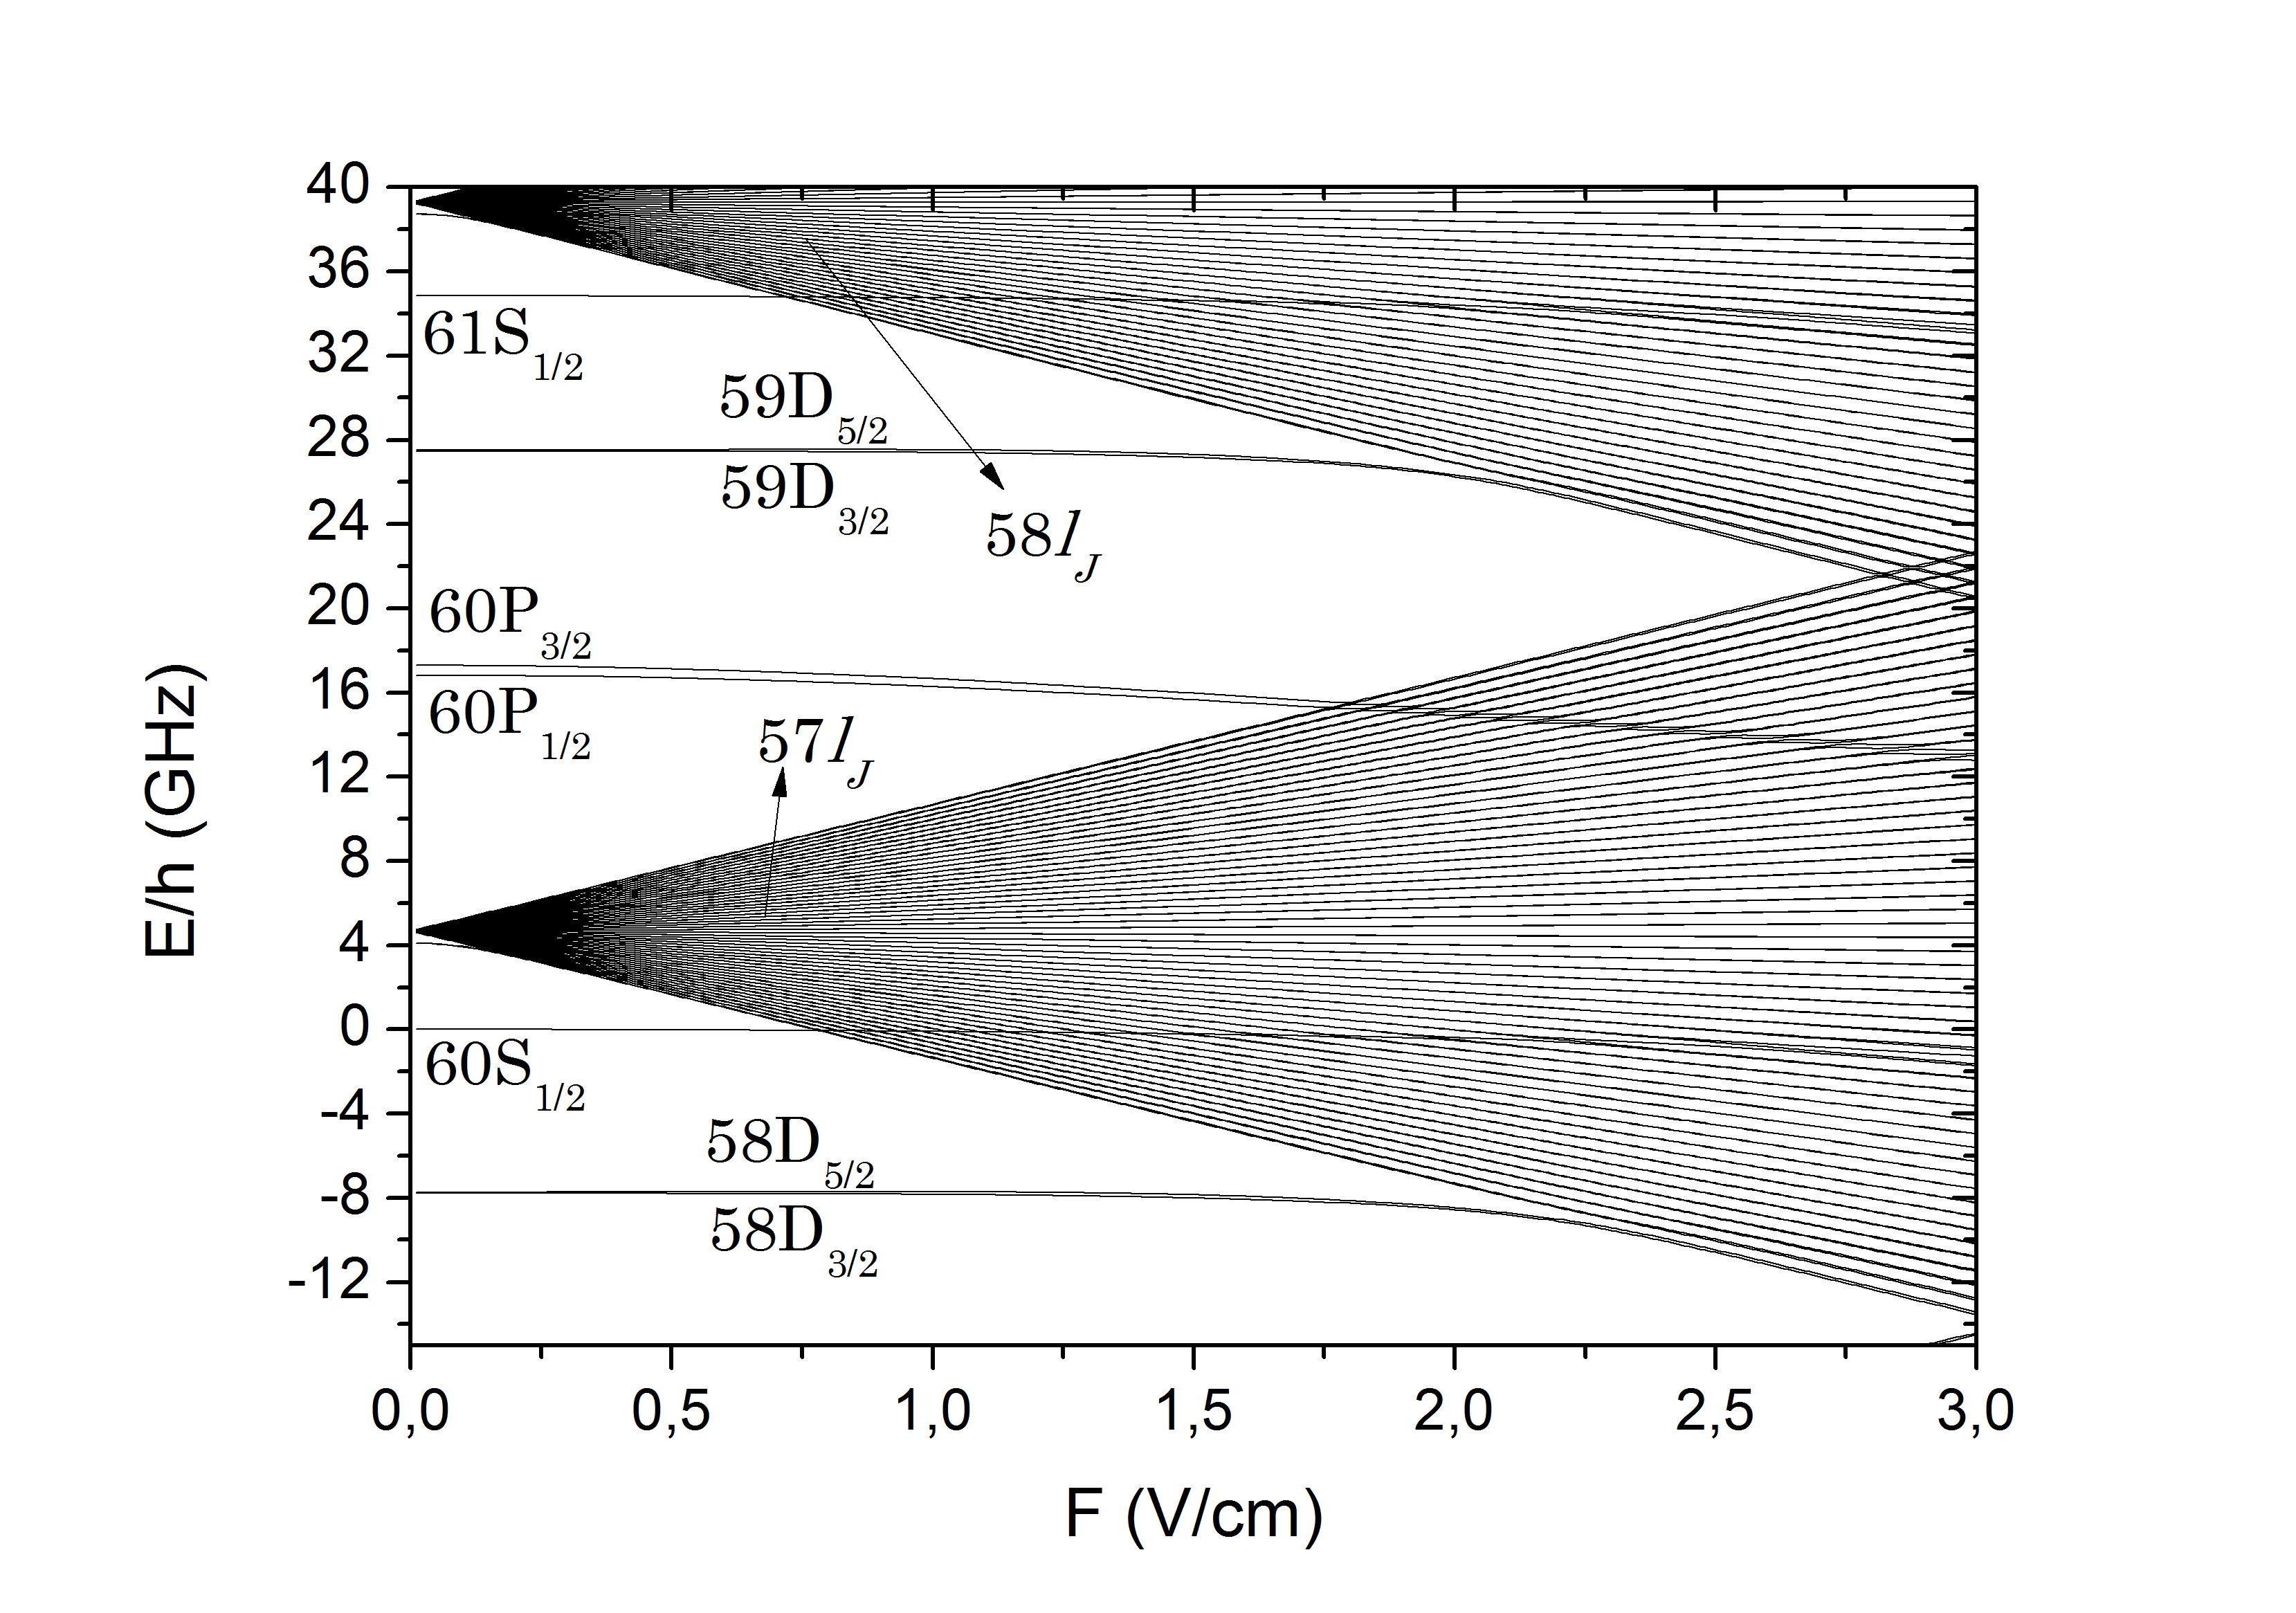
\includegraphics[width=\linewidth]{figures/Stark_60S}
\caption[Diagramme Stark autour du niveau $\mathrm{60S}$]{
Diagramme Stark autour du niveau $\mathrm{60S}$, pour les états de $m_j=1/2$.
Le défaut quantique déplace beaucoup les niveaux S,P et D.
Ces niveaux non-dégénérés ont un effet Stark quadratique en champ électrique.
Les niveaux de grand $l$ sont dégénérés et ont un effet Stark linéaire (ce sont les multiplicités qui s'ouvrent en éventail).
}
\label{fig:Stark_60S}
\end{figure}
%
Deux cas sont à distinguer. Les niveaux de faible moment orbital $l\leq 3$ sont déplacés en énergie par leur défaut quantique important.
Le terme d'interaction Stark ne couplant que des niveaux ayant la même énergie en l'absence de champ électrique, ces niveaux S,P et D ne sont perturbés qu'au second ordre par l'effet Stark.
Leur énergie varie donc de façon quadratique avec le champ électrique.
Les niveaux de grand nombre quantique orbital $l$ et de même nombre quantique principal $n$ sont, eux, dégénérés.
Le champ électrique sépare donc leurs énergies linéairement
\footnote{
Le cas de l'effet Stark pour les atomes de grand $l$ sera traité plus en détail dans le chapitre \ref{chapter:circsim}.
}.
La figure \eqref{fig:Stark_60S} montre deux telles multiplicités, $n=57$ et $n=58$.

Les niveaux de bas $l$ présentent donc tous un effet Stark quadratique que l'on exprime sous la forme
\begin{equation}
\label{eq:Stark_quad}
\Delta \nu_S = A.\vec{F}^2
\end{equation}
On comprend mieux ainsi la forme des raies présentées en figure \eqref{fig:vieilles_raies} :
l'effet Stark ne peut que réduire la fréquence de transition $5S-60S$ et la raie n'est donc élargie que du côté des basses fréquences.

La diagonalisation du hamiltonien \eqref{eq:hamilt_Stark} et l'ajustement des énergies propres ainsi calculées nous permettent d'extraire les coefficients d'effet Stark pour n'importe quel niveau.
La table \eqref{tab:Stark_60S} repertorie les coefficients d'effet Stark quadratique pour quelques niveaux autour du $\mathrm{60S}$.

\begin{table}[h]
	\centering
	\caption[Effet Stark quadratique des niveaux proches du $\mathrm{60S}$]{Coefficients d'effet Stark quadratique de niveaux proches du $\mathrm{60S}$.
	}
	\label{tab:Stark_60S}
	\begin{tabular}{c c }
		\toprule\midrule
		Niveau de Rydberg
		& Coefficient Stark quadratique
		\\
		$\ket{n,l,j}$
		& $A_{n,l,j,m_j}$ en $\si{\MHz \per (\V \per\cm) \squared}$ \\
		\midrule
		$\mathrm{60S_{1/2}}$
		& \SI{-89.9}{} \\
		$\mathrm{61S_{1/2}}$
		& \SI{-100.9}{} \\
		$\mathrm{60P_{3/2},m_j=\pm -1/2}$
		& \SI{-676}{} \\
		$\mathrm{60P_{3/2},m_j=\pm -3/2}$
		& \SI{-569}{} \\
		\midrule
		\bottomrule
 	\end{tabular}
\end{table}

\noindent Si l'on suppose que la largeur des spectres de la figure \eqref{fig:vieilles_raies} est due principalement à l'effet Stark causé par des gradients de champ électrique, alors ceux-ci peuvent s'estimer grâce ax coefficients données en table \eqref{tab:Stark_60S}.
Une largeur de raie de $\SI{40}{\MHz}$ correspond à un champ électrique variant de $\SIrange{0}{0.667}{\V/\cm}$ sur l'extension du nuage.
Or le nuage utilisé pour ces spectres était un MOT de $\sim \SI{200}{\um}$ de diamètre, ce qui nous donne une valeur de gradient de champ électrique de l'ordre de $\SI{35}{(\V/\cm)\per\cm}$.

%DISCREPANCY avec Raul, qui trouve $14 V/cm^2$. Ca semble se corriger par un facteur $2\pi$ dans la largeur, qui viendrait du fait qu'il a appelé $\Delta\omega$ la largeur de raie au lieu de $\Dela \nu$.

\subsubsection*{Potentiel de contact du rubidium sur l'or et dépôt contrôlé}
\noindent La cause principale de l'inhomogénéité spatiale et temporelle des champs électriques est l'accumulation d'un dépôt d'atomes de rubidium sur la surface en or de la puce :
lorsque les atomes du piège sont relâchés à la fin de chaque séquence, une partie d'entre eux entre en contact avec la surface froide de la puce et s'y dépose.
Des dépôts volontaires d'atomes sur la puce, à partir de nuages piégés, nous ont confirmé l'importance de ce phénomène et de ses effets sur les spectres d'excitation laser.

L'accumulation d'atomes de rubidium sur la puce forme d'important dipôles électriques.
En effet, les niveaux de Fermi de l'or et du rubidium étant différents, lorsque les deux métaux sont mis en contact les électrons se déplacent de l'un à l'autre pour équilibrer les niveaux de Fermi.
Un potentiel électrostatique de contact est alors créé entre l'or et le rubidium.
La surface de la puce étant mise à la masse, ce sont les plaques de rubidium déposé qui se chargent à $\SI{2.5}{\V}$ environ.
Or le dépôt de rubidium depuis les nuages piégés est un processus lent et non contrôlé, sur des échelles de longueur de l'ordre du $\si{\mm}$.
Cela a pour conséquence un champ électrique variant dans le temps et inhomogène à une distance de la puce inférieure à quelques $\si{\mm}$.
C'est justement là que se trouve les atomes piégés que l'on souhaite exciter.

La solution que nous avons envisagée et mise en \oe uvre fut de saturer le dépôt de rubidium sur la puce, en faisant un dépôt contrôlé macroscopique sur une surface grande devant la région de piégeage.
Pour que cela fonctionne, il est important que le rubidium déposé reste métallique, non oxydé, et ne migre pas dans le cryostat en raison de différences de températures.
Ces contraintes nous ont décidés à faire le dépôt de rubidium à froid, lorsque le cryostat est sous vide et thermiquement stable.
Le dépôt de contrôlé a été réalisé grâce à l'installation de dispenseurs de rubidium dans le cryostat, orientés de façon à pouvoir couvrir la puce de rubidium métallique.
La figure \eqref{fig:depotRb} illustre qualitativement la structure des champs électriques au voisinage de la puce avant et après le dépôt de rubidium.
%
\begin{figure}[h]
\centering
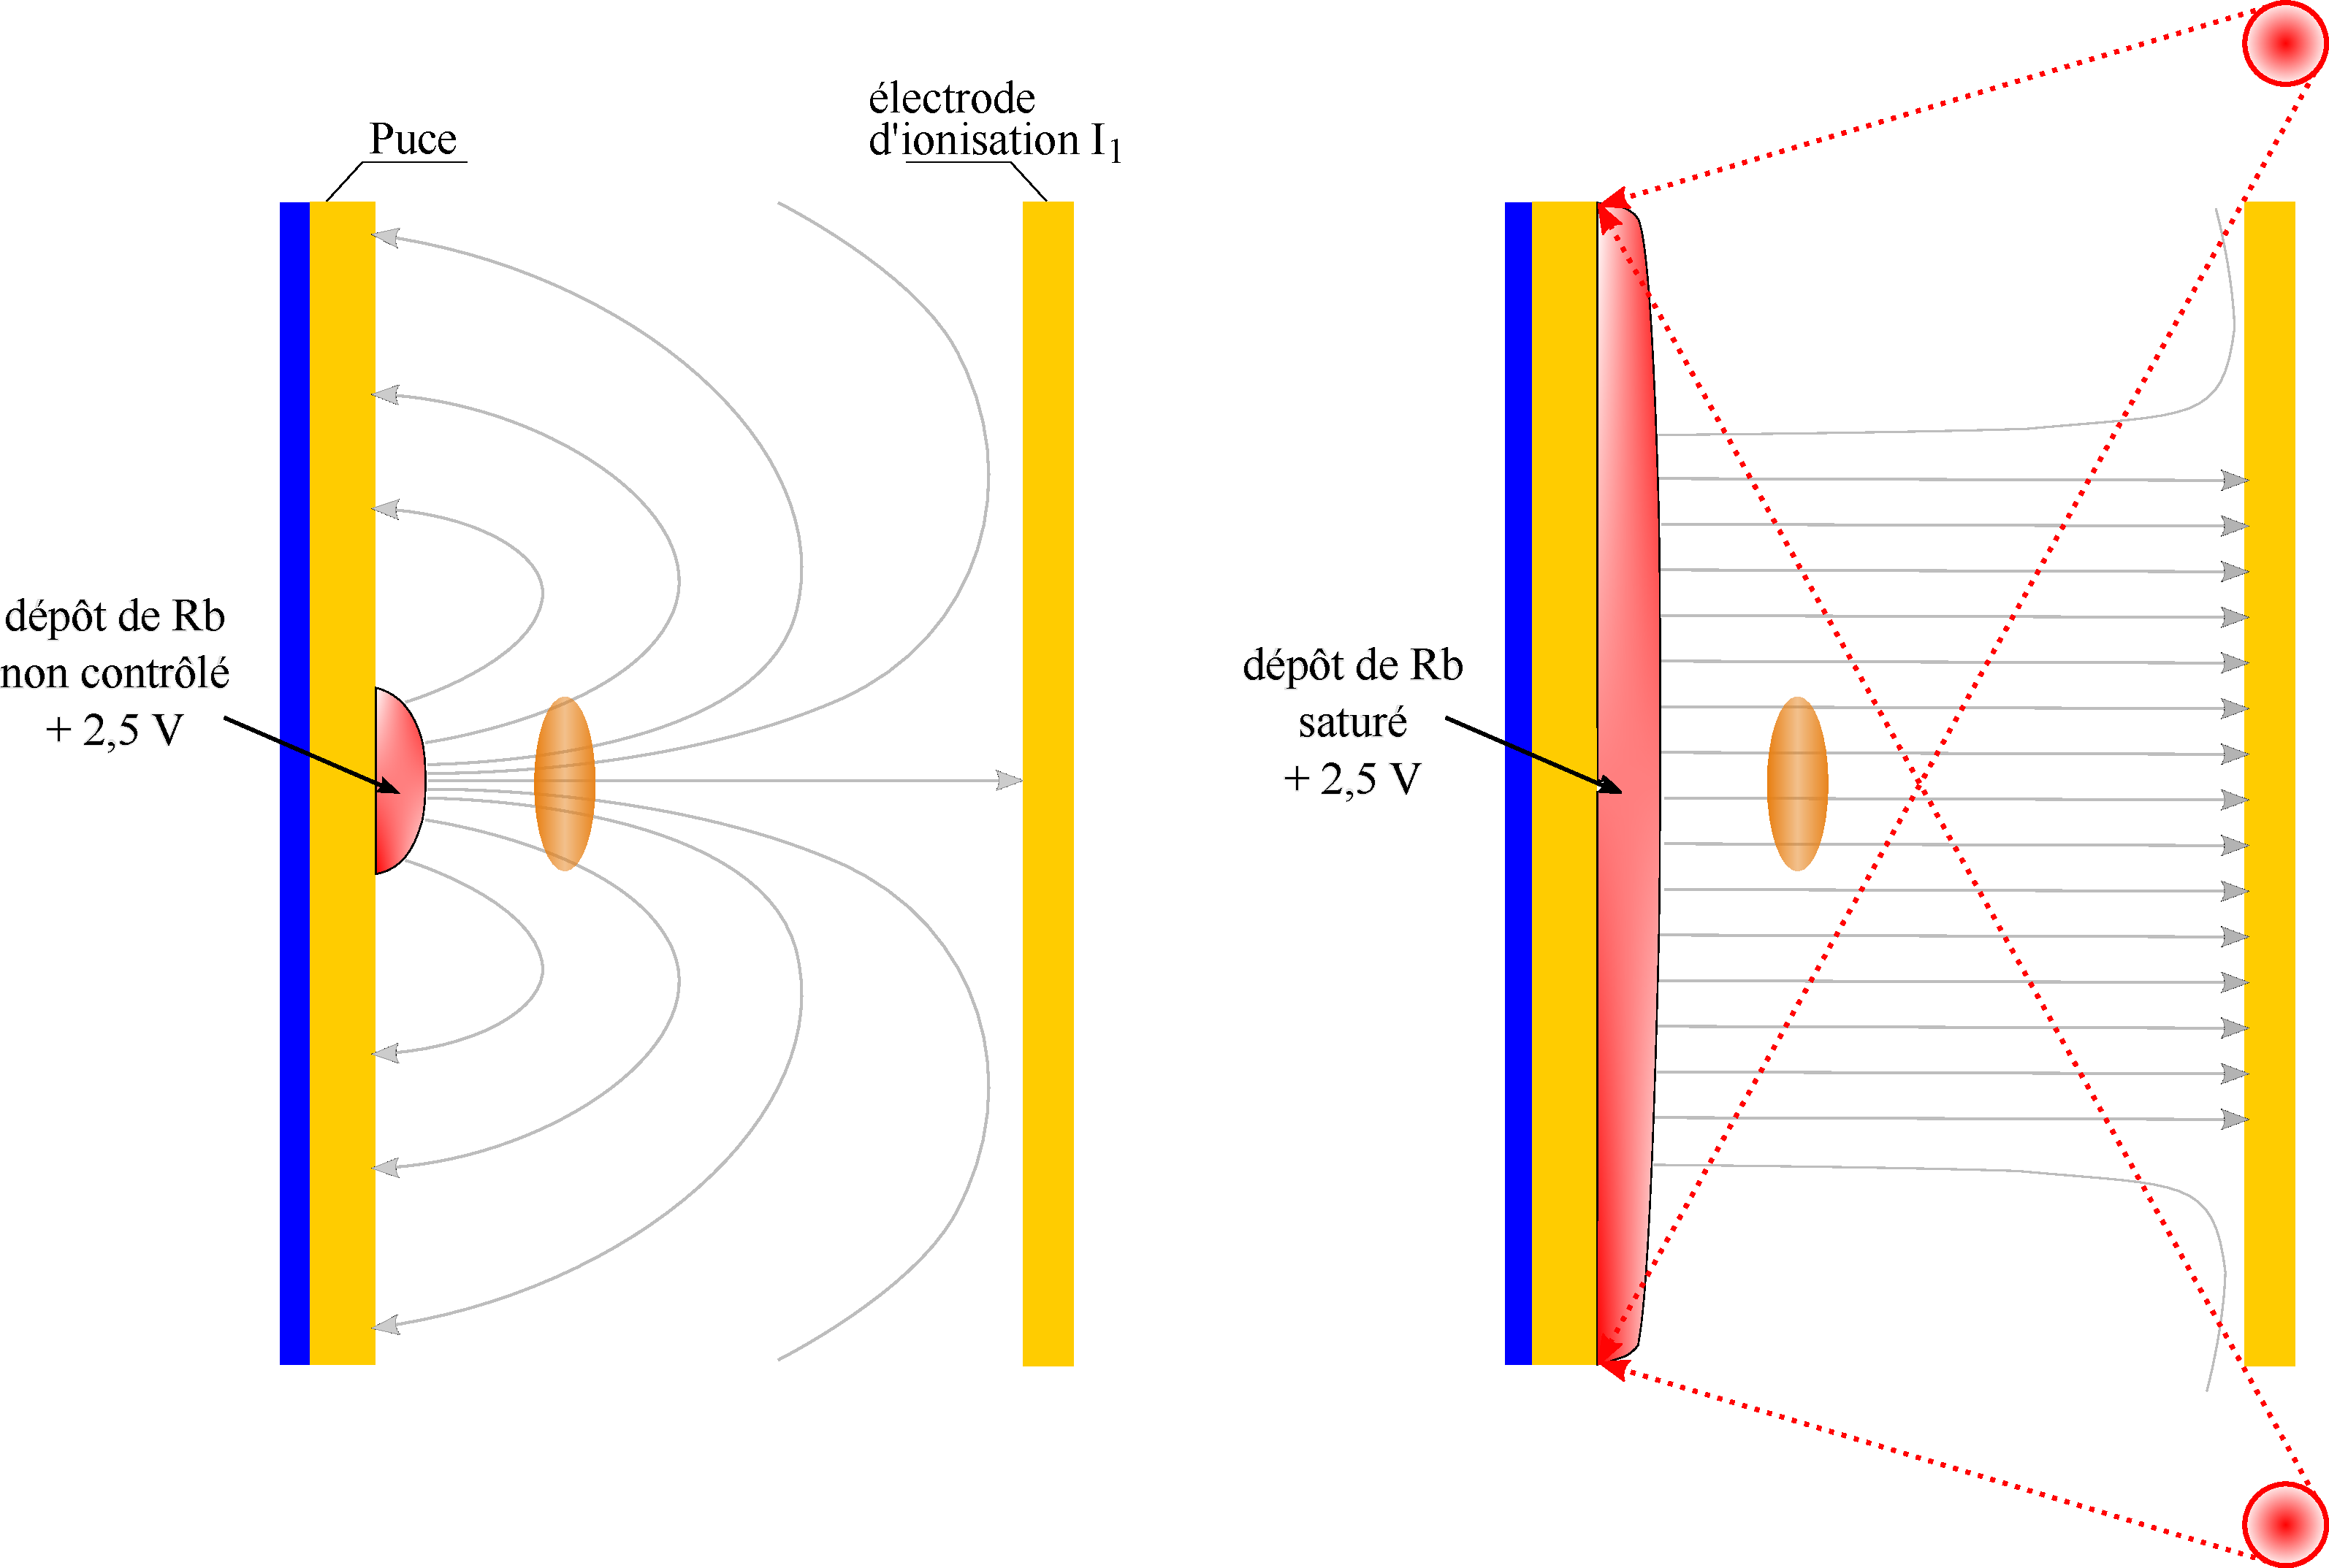
\includegraphics[width=.85\linewidth]{figures/depotRb}
\caption[Dépôt contrôlé de rubidium sur la puce]{
Schéma illustrant les dépôts de rubidium sur la puce et les champs électriques qui en résultent.
Les dépôts de rubidium sont représentés en rouge et les traits gris fléchés représentent les lignes de champ électrique
Les surfaces représentées en jaune (puce et électrode d'ionisation) sont mise à la masse.
L'ovale orange représente la position du nuage atomique (les échelles ne sont pas respéctées).
\`A gauche, dépôt non-contrôlé dû aux atomes piégés : le champ électrique est inhomogène  et varie dans le temps.
\`A droite, dépôt contrôlé réalisé grâce aux dispenseurs de rubidium (indiqués par les cercles rouges) : le champ électrique est homogène et stable dans le temps.
}
\label{fig:depotRb}
\end{figure}

Les dispenseurs nous ont permis de déposer une couche de rubidium, estimée à environ $\SI{80}{\nano\meter}$ d'épaisseur, sur une partie importante de la surface de la puce.
%Une telle épaisseur représente quelques centaines de mono-couches atomiques, et justifie que l'on puisse traiter le dépôt comme bulk metal

Un spectre d'excitation laser fait juste après ce dépôt de rubidium dans un MOT à $\SI{500}{\um}$ de la puce est présenté en figure \eqref{fig:raiefine_depot}.
Les conditions d'excitation sont similaires à celles des spectres présentés en figure \eqref{fig:vieilles_raies}, mais la largeur de raie spectrale est de seulement $\Delta\nu=\SI{1.7}{\MHz}$.
Le dépôt de rubidium a donc eu un effet extrêmement bénéfique sur l'excitation d'atomes de Rydberg au voisinage de la puce.
%
\begin{figure}[h]
\centering
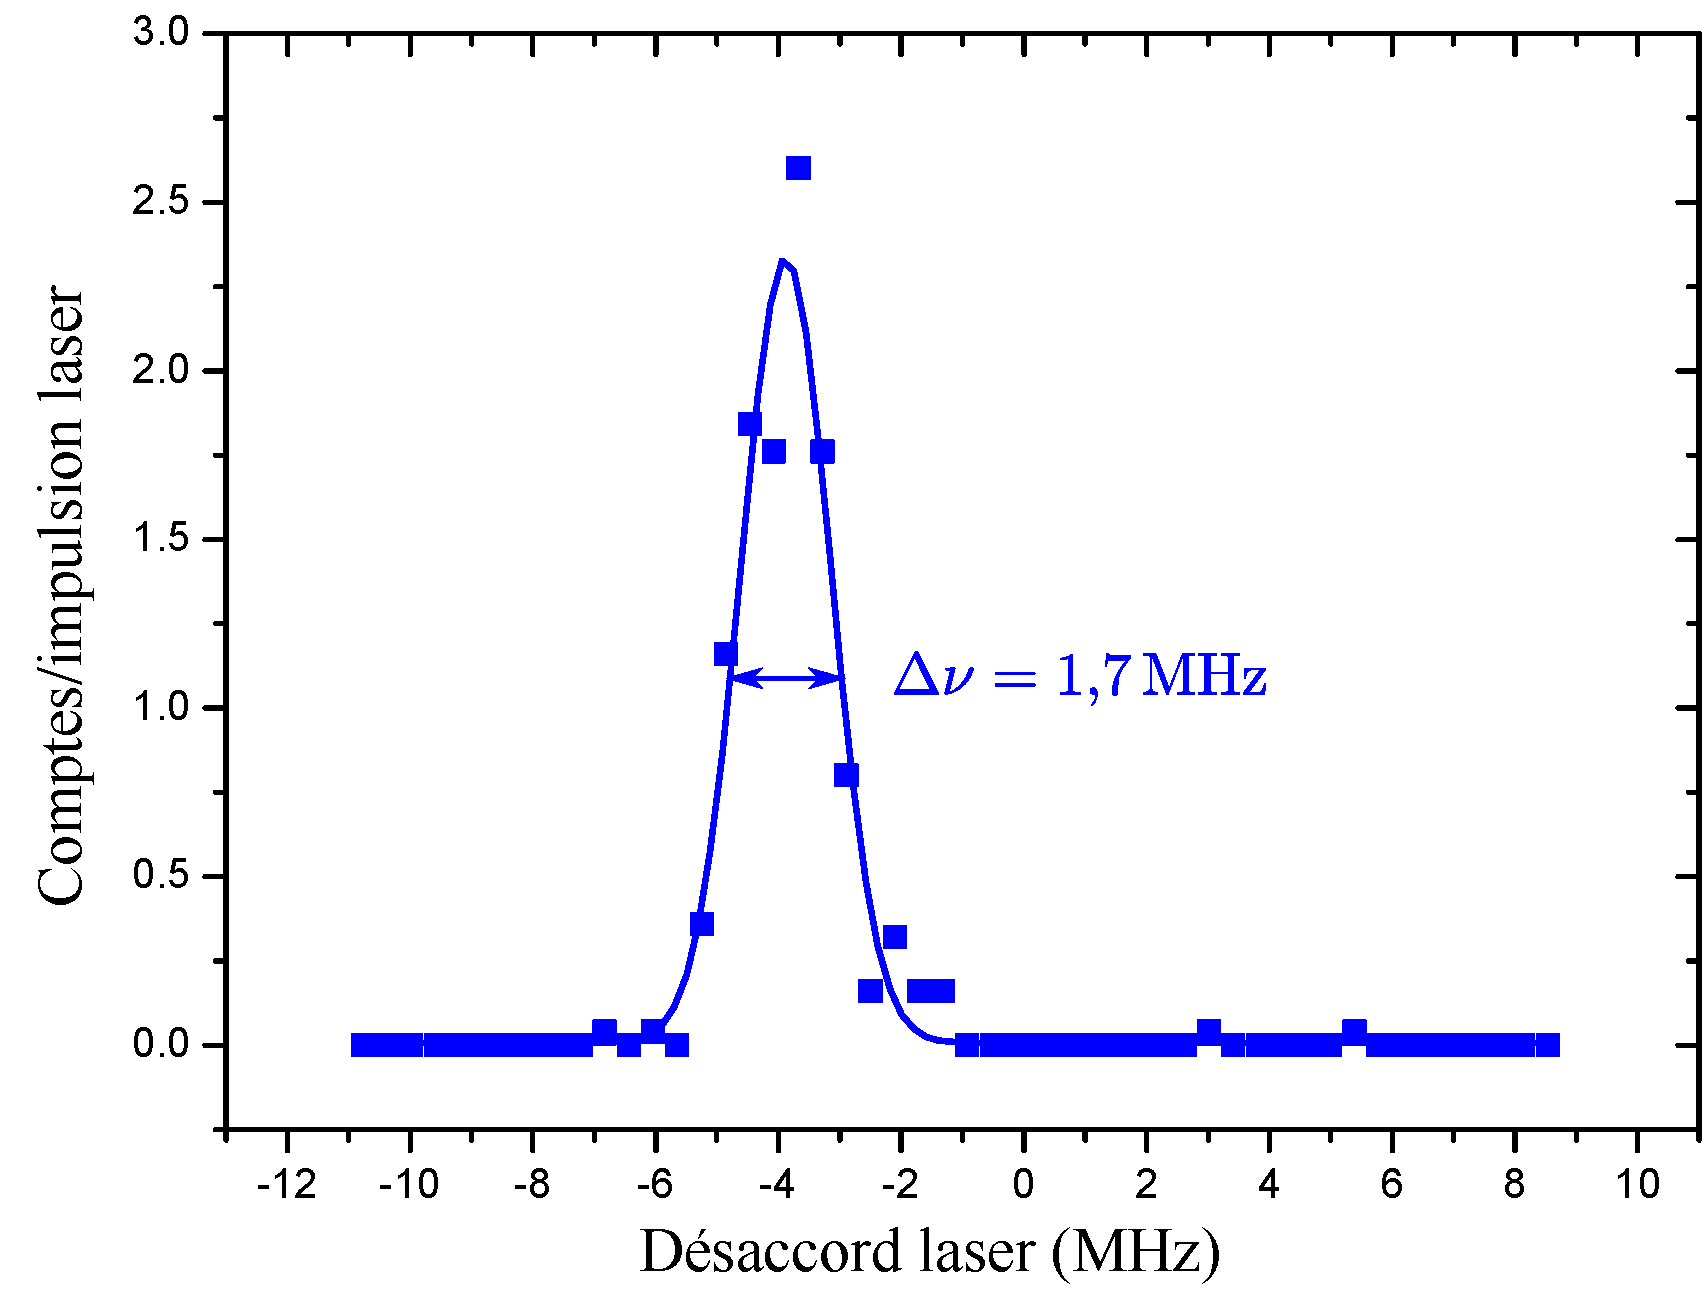
\includegraphics[width=.8\linewidth]{figures/raiefine_depot}
\caption[Spectre d'excitation laser 5S-60S juste après le dépôt de rubidium sur la puce]{
Spectre d'excitation laser 5S-60S d'atomes piégés dans un MOT, juste après le dépôt de rubidium sur la puce.
La largeur de raie a été considérablement réduite par le dépôt contrôlé de rubidium.
}
%

\label{fig:raiefine_depot}
\end{figure}

		
	\subsection{Contrôle du champ électrique}% et compensation}
\noindent Le dépôt saturé de rubidium sur la puce nous a permis de réduire considérablement les inhomogénéités de champ électrique.
% mais ne garantit en rien un champ nul
Nous souhaitons néanmoins pouvoir contrôler la valeur moyenne du champ à la position du nuage atomique, dans deux optiques.
La première est la réduction de l'effet des inhomogénéités résiduelles.
En effet, plus la valeur moyenne du champ électrique sera élevée, plus la raie spectrale sera élargie par une même variation autour de la valeur moyenne.
Cela est dû à la forme quadratique de l'effet Stark pour les niveaux de bas $l$, et se conçoit fort bien à l'observation de la figure \eqref{fig:Stark_60S}.
La seconde optique d'un contrôle plus fin du champ électrique est de pouvoir déplacer en fréquence la transition laser vers les niveaux de Rydberg ainsi que les transitions microonde entre niveaux de Rydberg voisins.
Cet aspect du contrôle des champs électriques nous sera surtout utile lorsque nous nous intéresserons aux niveaux de Rydberg circulaires, dans les chapitres \ref{chapter:circsim} et \ref{chapter:50c}.
	
Le moyen le plus direct dont nous disposons pour le contrôle du champ électrique est l'application d'une tension sur les électrodes d'ionisation $I_1$ et $I_2$ représentées en figure \eqref{fig:schema_detect}.
Il est raisonnable de supposer, étant donner la grande surface de ces électrodes, que le champ créé entre celles-ci et la puce sera spatialement homogène, au moins là où se situe le nuage atomique.
Le contrôle de la tension appliquée à ces électrodes présente une exigence technique particulière :
%demande un certain raffinement technique :
nous voulons contrôler le champ électrique vu par les atomes à l'échelle de la dizaine de $\si{\mV/\cm}$, tout en étant capable d'appliquer une tension de quelques centaines de Volts sur les mêmes électrodes afin d'ioniser et détecter les atomes de Rydberg.

Nous avons pour cela conçu un circuit électronique permettant de commuter rapidement la tension appliquée aux électrodes, entre une voie basse tension à bas bruit pendant l'excitation des atomes de Rydberg et une voie haute tension servant à leur détection.
Ce circuit est schématisé en figure \eqref{fig:detectionbox_ENS}.
%
\begin{figure}[h]
\centering
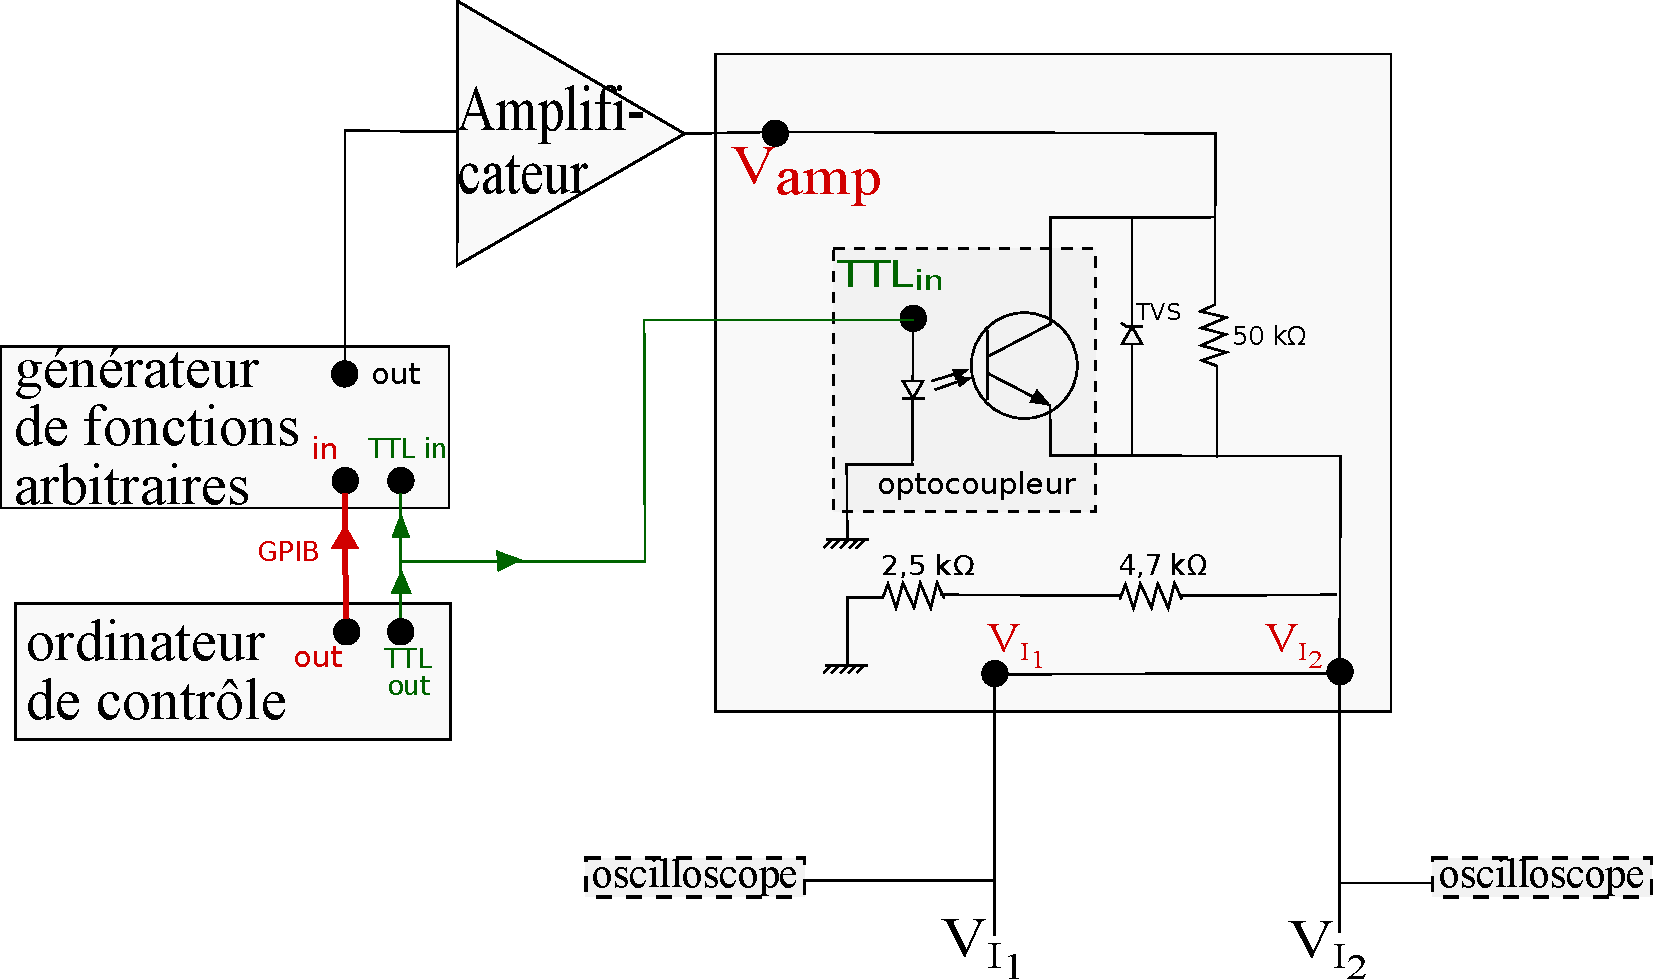
\includegraphics[width=.8\linewidth]{figures/detectionbox_ENS}
\caption[Premier circuit de contrôle de la tension des électrodes d'ionisation]{
Premier circuit de contrôle de la tension des électrodes d'ionisation.
Les tensions sont fournies par un générateur de fonctions arbitraires contrôlé par ordinateur, puis amplifiées par un amplificateur haute tension de gain $\times \num{50}$.
Pendant l'excitation des atomes de Rydberg, l'optocoupleur est bloquant.
Le pont diviseur de tension créé par la résistance de $\SI{50}{\kilo\ohm}$ d'une part et de $\SI{2.5}{} + \SI{4.7}{\kilo\ohm}$ divise par un facteur $\num{8}$ le bruit électronique au niveau des électrodes, au prix d'une réduction d'autant du signal.
Pendant la phase de détection, l'optocoupleur est passant et le pont diviseur est ainsi court-circuité.
La tension appliquée aux électrodes est alors directement la tension en sortie de l'amplificateur.
}
\label{fig:detectionbox_ENS}
\end{figure}
%

Toutes les expériences que nous décrirons dans la suite de cette thèse ayant trait au niveau $\mathrm{60S}$ ont été réalisées à l'aide de ce circuit.
Une particularité de son fonctionnement réside dans le fait que la phase d'excitation des atomes de Rydberg se fait à tension constante, et que le contrôle dynamique de la tension n'est permis que lors de la phase de détection, qui nécessite une rampe de tension comme évoqué en \ref{subsec:detection}.
Cette limitation sera corrigée plus tard par l'introduction d'un second circuit de contrôle, représenté en figure \eqref{fig:detectionbox_CdF} et son fonctionnement est détaillé ci-après.
Ce second circuit, qui permet l'application de deux rampes de tensions indépendantes pour l'excitation et la détection, a été utilisé dans toutes les éxpériences que nous décrirons ayant trait au niveau circulaire $\mathrm{50C}$.
%
\begin{figure}[h]
\centering
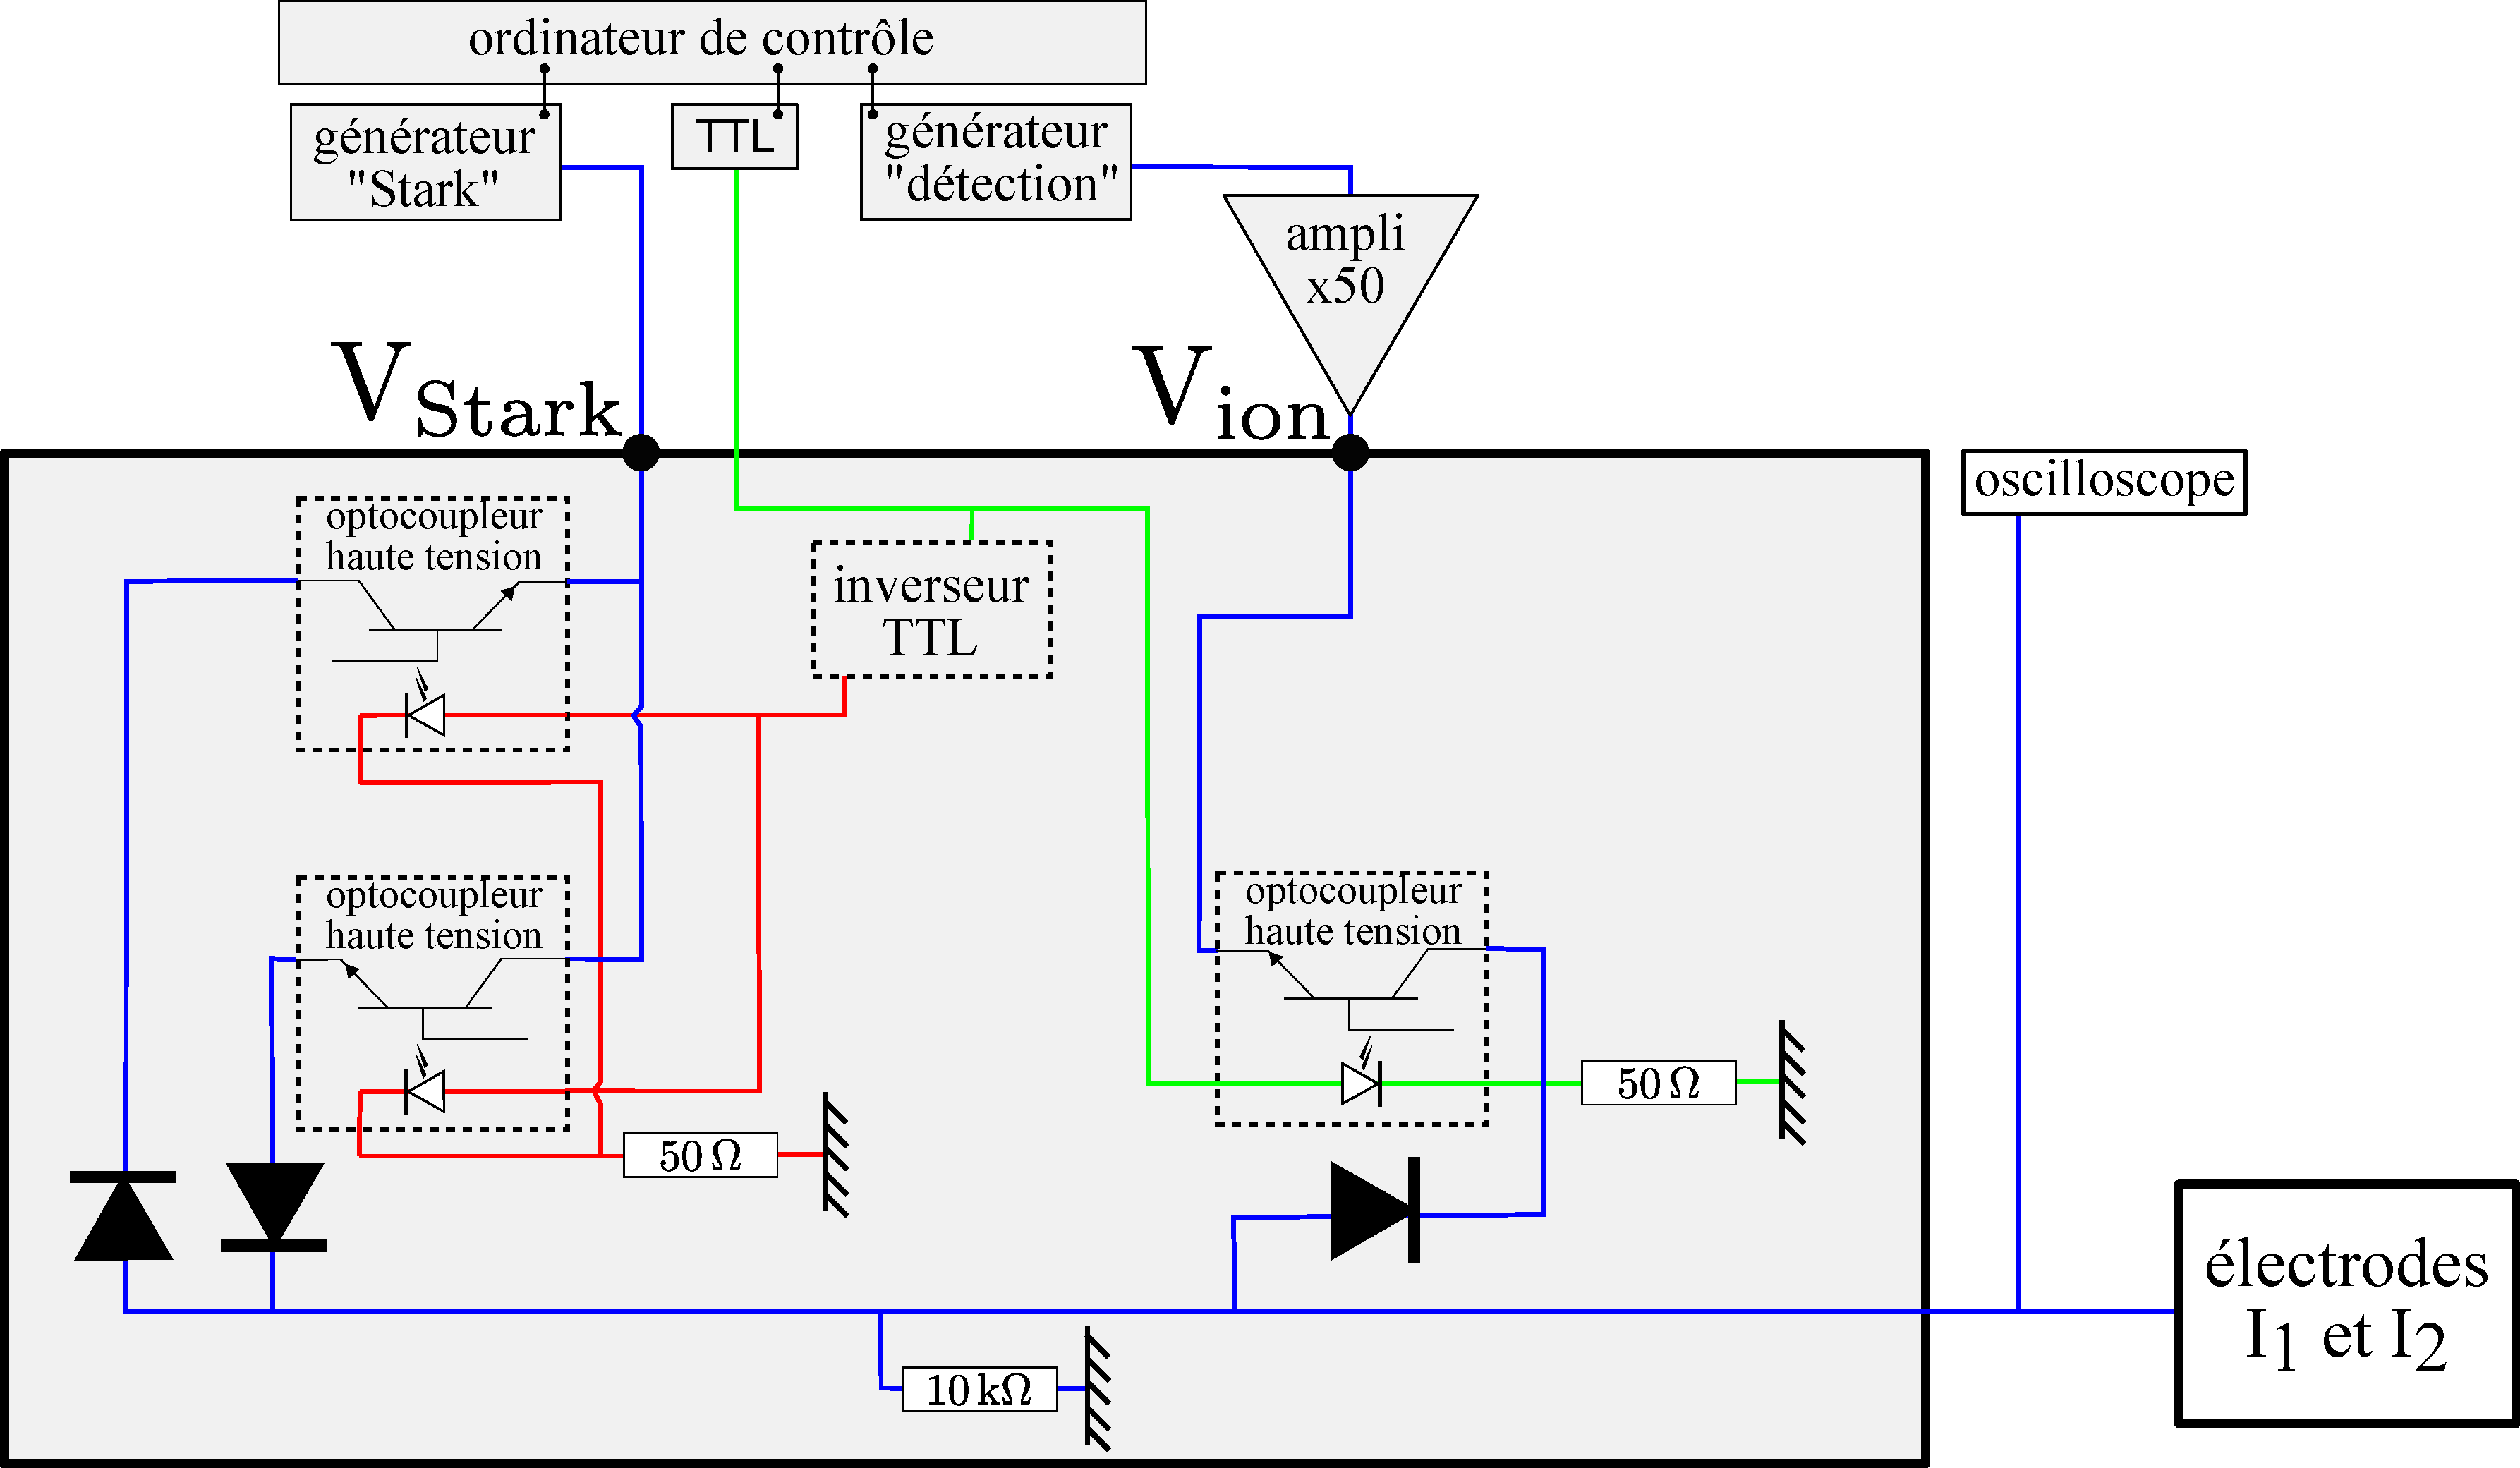
\includegraphics[width=\linewidth]{figures/detectionbox_CdF}
\caption[Second circuit de contrôle de la tension des électrodes d'ionisation]{
Second circuit de contrôle de la tension des électrodes d'ionisation.
Les tensions sont fournies par deux générateurs de fonctions arbitraires indépendants et appliquées directement aux électrodes par deux voies séparées (voie basse tension à gauche et voie haute tension à droite).
}
\label{fig:detectionbox_CdF}
\end{figure}

Dans ce second circuit de contrôle de tension, l'ordinateur de contrôle permet de programmer une rampe arbitraire sur chacun des générateurs.
La tension fournie par le générateur \og détection \fg{} est amplifiée $\num{50}$ fois et devient \og $\mathrm{V_{ion}}$ \fg{}.
$\mathrm{V_{ion}}$ est introduite dans la voie haute tension du circuit de contrôle.
La tension fournie par le générateur \og Stark \fg{} n'est pas amplifiée et est appelée \og $\mathrm{V_{Stark}}$ \fg{}.
$\mathrm{V_{Stark}}$ est introduite dans la voie basse tension du circuit de contrôle.
Pendant la phase d'excitation, le signal TTL est éteint. L'optocoupleur de la voie haute tension est alors bloquant, et les deux optocoupleurs de la voie basse tension sont passants.
L'optocoupleur du haut sert à faire passer les tension négatives et celui du bas les tensions positives.
Chacun est isolé par une diode à sa sortie, adaptée au sens de circulation du courant dans chaque voie.
La tension $\mathrm{V_{Stark}}$ est alors directement appliquée aux électrodes.
Pendant la phase de détection, le signal TTL est allumé. Les optocoupleurs de la voie basse tension deviennent bloquants et celui de la voie haute tension devient passant.
La tension $\mathrm{V_{ion}}$ est alors directement appliquée aux électrodes.
Les tensions en fin de rampe de détection peuvent aller de $\SI{-150}{\V}$ pour les niveaux voisins du $\mathrm{60S}$, et jusqu'à $\SI{-500}{\V}$ pour les niveaux voisins du $\mathrm{50C}$.
Nous avons donc conçu ce circuit de contrôle en conséquence, en utilisant des optocoupleurs capables de bloquer des tensions élevées.
	
 \subsubsection*{Contrôle du champ parallèle à la puce et électrodes de circularisation}
\noindent Les dispositifs de contrôle des champs électriques que nous venons de présenter ont une lacune majeure :
ils ne permettent de varier le champ électrique que perpendiculairement à la puce, soit dans la direction $y$.
Lorsque nous avons commencé à travailler dans l'optique d'obtenir des atomes de Rydberg circulaires, nous avons souhaité pouvoir contrôler le champ électrique parallèlement à la puce.
Cela a deux conséquences.
En premier lieu, nous serons en mesure de compenser les champs résiduels dans les directions $x$ et $z$.
En second lieu, cela permettra d'appliquer un champ électrique radio-fréquence polarisé, nécessaire à la circularisation des niveaux de Rydberg, qui sera discutée au chapitre \ref{chapter:50c}.


Notre dispositif de contrôle du champ parallèle à la puce consiste en quatre électrodes cylindriques (\og électrodes RF \fg{}) , disposées en carré autour de la zone de piégeage des atomes.
La figure \ref{fig:RF_ELECTRODES} montre la disposition de ces électrodes au c\oe ur du dispositif expérimental.
%
\begin{figure}[h]
\centering
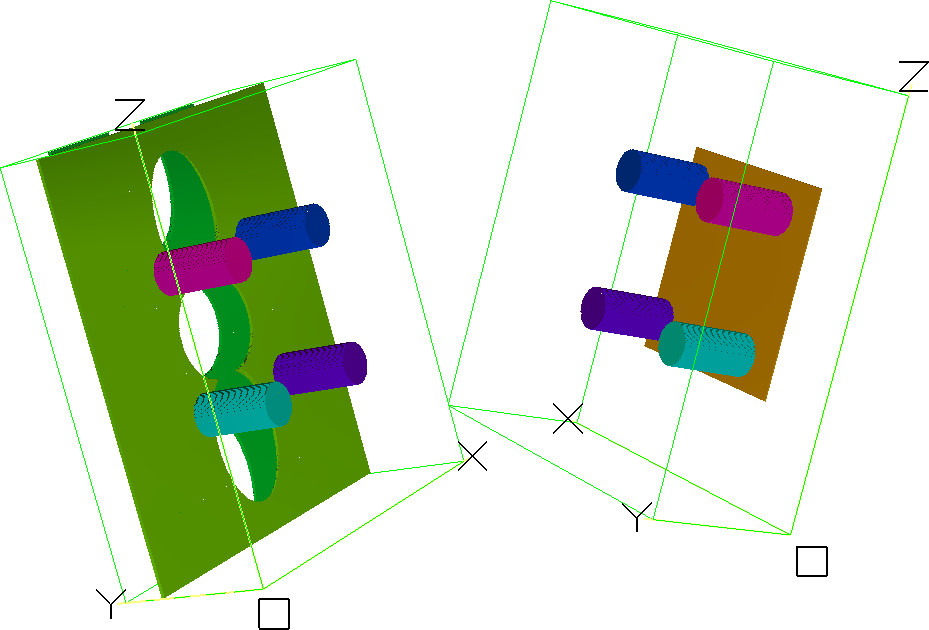
\includegraphics[width=\linewidth]{figures/RF_electrodes}
\caption[Électrodes de circularisation et de contrôle du champ parallèle]{
Électrodes \og RF \fg{} de circularisation et de contrôle du champ parallèle à la puce.
}
\label{fig:RF_ELECTRODES}
\end{figure}
%
En appliquant des tensions arbitraires sur ces électrodes, nous pourrons compenser les champs résiduels dans les directions $x$ et $z$, et espérer compenser même les gradients de champ dans ces directions.
En leur appliquant des tensions oscillant à une fréquence de $\SI{230}{\MHz}$ avec avec des phases bien optimisés, nous pourrons générer un champ électrique radio-fréquence arbitrairement polarisé au niveau des atomes.

\bigskip
\noindent rentrer dans une description détaillée de la géométrie et donner des résultats de SIMION ? nécessaire ou pas ?


\newpage
	\subsection{manipulation et observation des Rydbergs}
\noindent C'est bien de détecter des Rydberg, mais il faut aussi pouvoir les manipuler et les caractériser.
Pour ça, on a un outil fabuleux : la spectroscopie microonde vers les niveaux voisins ! \\
schéma de niveaux ? schéma de dispositif ? \\
on peut mentionner ici qu'avec ça on a pu calibrer les champs électriques résiduels, et faire un qubit $60s-61s$ qui vit très longtemps.

\section*{Conclusion}
On a un dispositif lourd et complexe mais qui permet de faire beaucoup de belles choses avec des Rydbergs ultra-froids.